\section{Methods} \label{sec:model}

In this section, we describe our baseline approaches, deliberation and LAS-JATD, as well as the proposed Deliberation-JATD method.

\subsection{Baseline Approaches}

\subsubsection{Deliberation}
\label{sec:methods_delib}


\begin{figure}[h!]
\begin{center}

\centering \scalebox{0.8}{
\ifx\du\undefined
  \newlength{\du}
\fi
\setlength{\du}{15\unitlength}
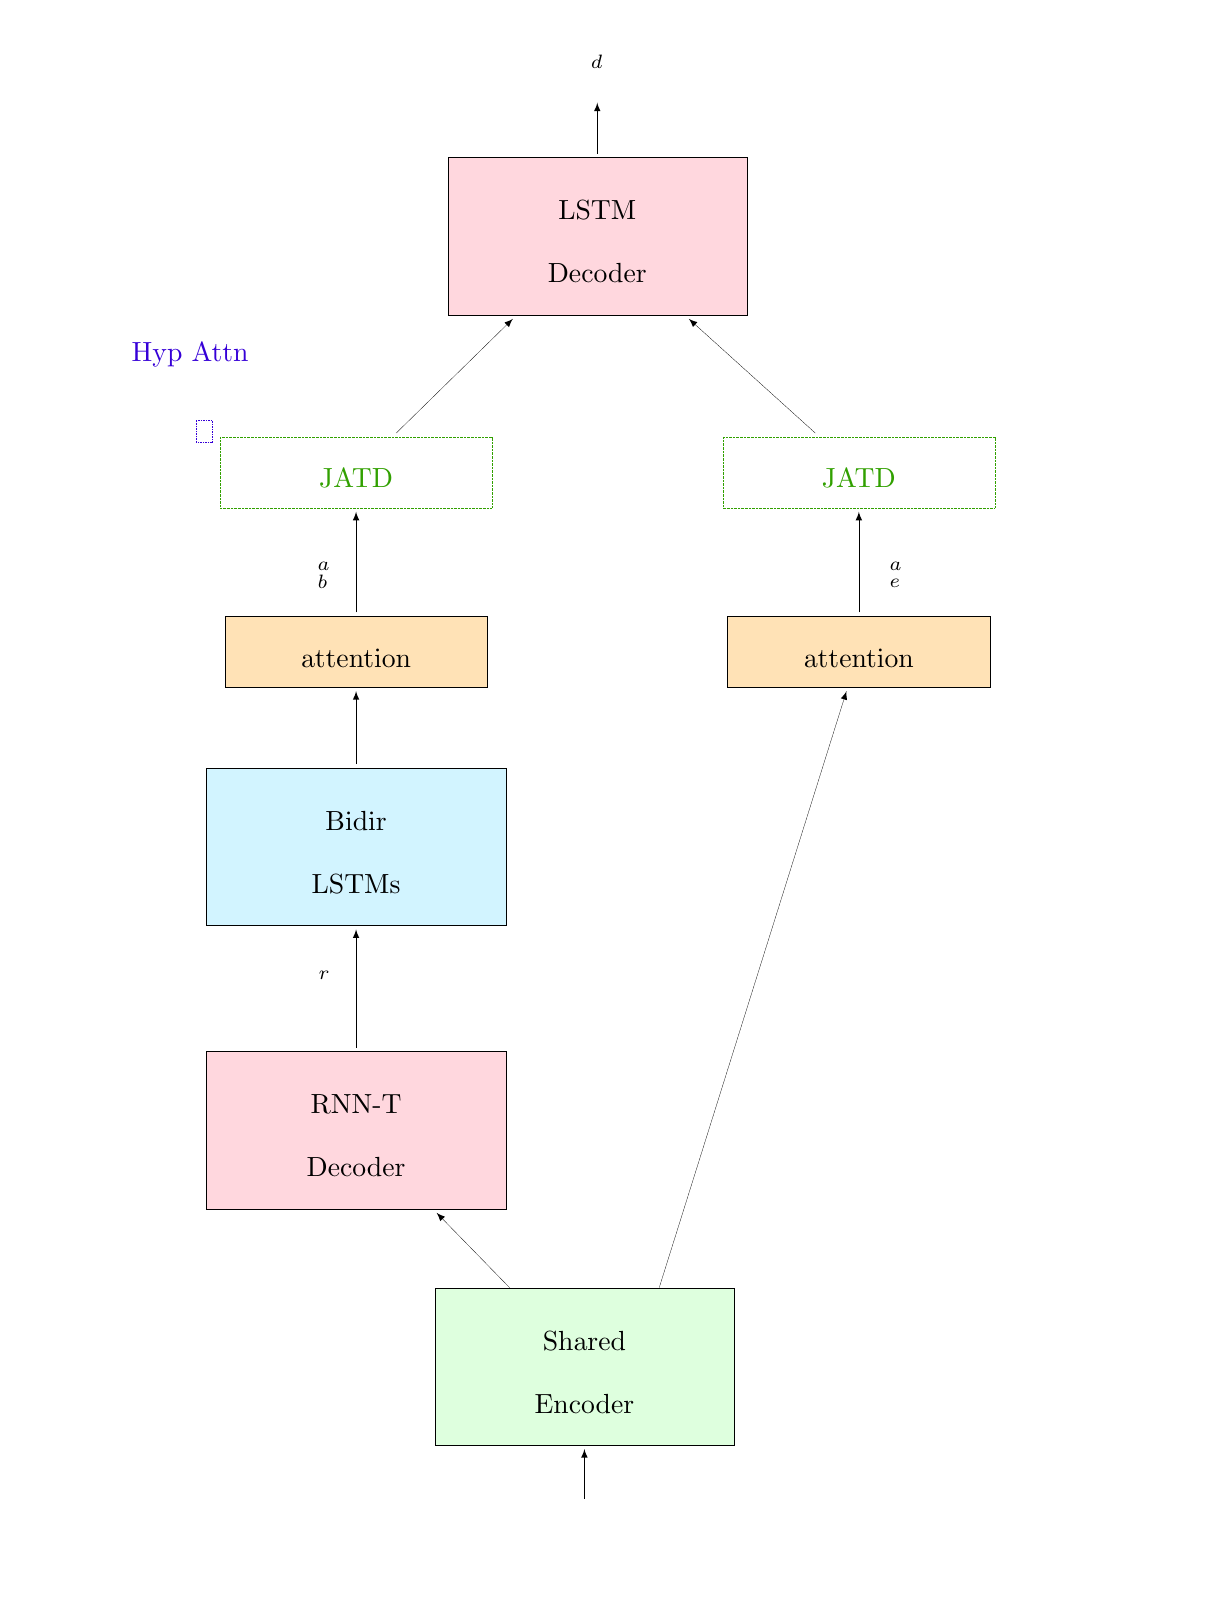
\begin{tikzpicture}[even odd rule]
\pgftransformxscale{1.000000}
\pgftransformyscale{-1.000000}
\definecolor{dialinecolor}{rgb}{0.000000, 0.000000, 0.000000}
\pgfsetstrokecolor{dialinecolor}
\pgfsetstrokeopacity{1.000000}
\definecolor{diafillcolor}{rgb}{1.000000, 1.000000, 1.000000}
\pgfsetfillcolor{diafillcolor}
\pgfsetfillopacity{1.000000}
\pgfsetlinewidth{0.100000\du}
\pgfsetdash{{0.300000\du}{0.300000\du}}{0\du}
\pgfsetmiterjoin
\pgfsetbuttcap
\definecolor{diafillcolor}{rgb}{1.000000, 1.000000, 1.000000}
\pgfsetfillcolor{diafillcolor}
\pgfsetfillopacity{0.000000}
\definecolor{dialinecolor}{rgb}{0.211765, 0.000000, 0.843137}
\pgfsetstrokecolor{dialinecolor}
\pgfsetstrokeopacity{1.000000}
\pgfpathmoveto{\pgfpoint{-0.800000\du}{7.591290\du}}
\pgfpathlineto{\pgfpoint{4.800000\du}{7.591290\du}}
\pgfpathlineto{\pgfpoint{4.800000\du}{-0.600000\du}}
\pgfpathlineto{\pgfpoint{-0.800000\du}{-0.600000\du}}
\pgfpathlineto{\pgfpoint{-0.800000\du}{7.591290\du}}
\pgfpathclose
\pgfusepath{fill,stroke}
\pgfsetlinewidth{0.100000\du}
\pgfsetdash{}{0pt}
\pgfsetmiterjoin
{\pgfsetcornersarced{\pgfpoint{0.000000\du}{0.000000\du}}\definecolor{diafillcolor}{rgb}{1.000000, 0.843137, 0.870588}
\pgfsetfillcolor{diafillcolor}
\pgfsetfillopacity{1.000000}
\fill (0.100000\du,8.000000\du)--(0.100000\du,10.000000\du)--(3.900000\du,10.000000\du)--(3.900000\du,8.000000\du)--cycle;
}{\pgfsetcornersarced{\pgfpoint{0.000000\du}{0.000000\du}}\definecolor{dialinecolor}{rgb}{0.000000, 0.000000, 0.000000}
\pgfsetstrokecolor{dialinecolor}
\pgfsetstrokeopacity{1.000000}
\draw (0.100000\du,8.000000\du)--(0.100000\du,10.000000\du)--(3.900000\du,10.000000\du)--(3.900000\du,8.000000\du)--cycle;
}% setfont left to latex
\definecolor{dialinecolor}{rgb}{0.000000, 0.000000, 0.000000}
\pgfsetstrokecolor{dialinecolor}
\pgfsetstrokeopacity{1.000000}
\definecolor{diafillcolor}{rgb}{0.000000, 0.000000, 0.000000}
\pgfsetfillcolor{diafillcolor}
\pgfsetfillopacity{1.000000}
\node[anchor=base,inner sep=0pt, outer sep=0pt,color=dialinecolor] at (2.000000\du,8.794062\du){RNN-T};
% setfont left to latex
\definecolor{dialinecolor}{rgb}{0.000000, 0.000000, 0.000000}
\pgfsetstrokecolor{dialinecolor}
\pgfsetstrokeopacity{1.000000}
\definecolor{diafillcolor}{rgb}{0.000000, 0.000000, 0.000000}
\pgfsetfillcolor{diafillcolor}
\pgfsetfillopacity{1.000000}
\node[anchor=base,inner sep=0pt, outer sep=0pt,color=dialinecolor] at (2.000000\du,9.594062\du){Decoder};
\pgfsetlinewidth{0.100000\du}
\pgfsetdash{}{0pt}
\pgfsetmiterjoin
{\pgfsetcornersarced{\pgfpoint{0.000000\du}{0.000000\du}}\definecolor{diafillcolor}{rgb}{1.000000, 0.843137, 0.870588}
\pgfsetfillcolor{diafillcolor}
\pgfsetfillopacity{1.000000}
\fill (3.163380\du,-3.354300\du)--(3.163380\du,-1.354300\du)--(6.963380\du,-1.354300\du)--(6.963380\du,-3.354300\du)--cycle;
}{\pgfsetcornersarced{\pgfpoint{0.000000\du}{0.000000\du}}\definecolor{dialinecolor}{rgb}{0.000000, 0.000000, 0.000000}
\pgfsetstrokecolor{dialinecolor}
\pgfsetstrokeopacity{1.000000}
\draw (3.163380\du,-3.354300\du)--(3.163380\du,-1.354300\du)--(6.963380\du,-1.354300\du)--(6.963380\du,-3.354300\du)--cycle;
}% setfont left to latex
\definecolor{dialinecolor}{rgb}{0.000000, 0.000000, 0.000000}
\pgfsetstrokecolor{dialinecolor}
\pgfsetstrokeopacity{1.000000}
\definecolor{diafillcolor}{rgb}{0.000000, 0.000000, 0.000000}
\pgfsetfillcolor{diafillcolor}
\pgfsetfillopacity{1.000000}
\node[anchor=base,inner sep=0pt, outer sep=0pt,color=dialinecolor] at (5.063380\du,-2.560237\du){LSTM};
% setfont left to latex
\definecolor{dialinecolor}{rgb}{0.000000, 0.000000, 0.000000}
\pgfsetstrokecolor{dialinecolor}
\pgfsetstrokeopacity{1.000000}
\definecolor{diafillcolor}{rgb}{0.000000, 0.000000, 0.000000}
\pgfsetfillcolor{diafillcolor}
\pgfsetfillopacity{1.000000}
\node[anchor=base,inner sep=0pt, outer sep=0pt,color=dialinecolor] at (5.063380\du,-1.760237\du){Decoder};
\pgfsetlinewidth{0.100000\du}
\pgfsetdash{}{0pt}
\pgfsetbuttcap
{
\definecolor{diafillcolor}{rgb}{0.000000, 0.000000, 0.000000}
\pgfsetfillcolor{diafillcolor}
\pgfsetfillopacity{1.000000}

\pgfsetarrowsend{latex}
\definecolor{dialinecolor}{rgb}{0.000000, 0.000000, 0.000000}
\pgfsetstrokecolor{dialinecolor}
\pgfsetstrokeopacity{1.000000}
\draw (2.000000\du,7.950146\du)--(2.000000\du,6.449854\du);
}
\pgfsetlinewidth{0.100000\du}
\pgfsetdash{}{0pt}
\pgfsetbuttcap
{
\definecolor{diafillcolor}{rgb}{0.000000, 0.000000, 0.000000}
\pgfsetfillcolor{diafillcolor}
\pgfsetfillopacity{1.000000}

\pgfsetarrowsend{latex}
\definecolor{dialinecolor}{rgb}{0.000000, 0.000000, 0.000000}
\pgfsetstrokecolor{dialinecolor}
\pgfsetstrokeopacity{1.000000}
\draw (5.063380\du,-3.402833\du)--(5.063380\du,-4.049856\du);
}
\pgfsetlinewidth{0.100000\du}
\pgfsetdash{}{0pt}
\pgfsetmiterjoin
{\pgfsetcornersarced{\pgfpoint{0.000000\du}{0.000000\du}}\definecolor{diafillcolor}{rgb}{0.870588, 1.000000, 0.870588}
\pgfsetfillcolor{diafillcolor}
\pgfsetfillopacity{1.000000}
\fill (3.000000\du,11.000000\du)--(3.000000\du,13.000000\du)--(6.800000\du,13.000000\du)--(6.800000\du,11.000000\du)--cycle;
}{\pgfsetcornersarced{\pgfpoint{0.000000\du}{0.000000\du}}\definecolor{dialinecolor}{rgb}{0.000000, 0.000000, 0.000000}
\pgfsetstrokecolor{dialinecolor}
\pgfsetstrokeopacity{1.000000}
\draw (3.000000\du,11.000000\du)--(3.000000\du,13.000000\du)--(6.800000\du,13.000000\du)--(6.800000\du,11.000000\du)--cycle;
}% setfont left to latex
\definecolor{dialinecolor}{rgb}{0.000000, 0.000000, 0.000000}
\pgfsetstrokecolor{dialinecolor}
\pgfsetstrokeopacity{1.000000}
\definecolor{diafillcolor}{rgb}{0.000000, 0.000000, 0.000000}
\pgfsetfillcolor{diafillcolor}
\pgfsetfillopacity{1.000000}
\node[anchor=base,inner sep=0pt, outer sep=0pt,color=dialinecolor] at (4.900000\du,11.794062\du){Shared};
% setfont left to latex
\definecolor{dialinecolor}{rgb}{0.000000, 0.000000, 0.000000}
\pgfsetstrokecolor{dialinecolor}
\pgfsetstrokeopacity{1.000000}
\definecolor{diafillcolor}{rgb}{0.000000, 0.000000, 0.000000}
\pgfsetfillcolor{diafillcolor}
\pgfsetfillopacity{1.000000}
\node[anchor=base,inner sep=0pt, outer sep=0pt,color=dialinecolor] at (4.900000\du,12.594062\du){Encoder};
\pgfsetlinewidth{0.100000\du}
\pgfsetdash{}{0pt}
\pgfsetbuttcap
{
\definecolor{diafillcolor}{rgb}{0.000000, 0.000000, 0.000000}
\pgfsetfillcolor{diafillcolor}
\pgfsetfillopacity{1.000000}

\pgfsetarrowsend{latex}
\definecolor{dialinecolor}{rgb}{0.000000, 0.000000, 0.000000}
\pgfsetstrokecolor{dialinecolor}
\pgfsetstrokeopacity{1.000000}
\draw (4.900000\du,13.682159\du)--(4.900000\du,13.049352\du);
}
\pgfsetlinewidth{0.100000\du}
\pgfsetdash{}{0pt}
\pgfsetbuttcap
{
\definecolor{diafillcolor}{rgb}{0.000000, 0.000000, 0.000000}
\pgfsetfillcolor{diafillcolor}
\pgfsetfillopacity{1.000000}

\pgfsetarrowsend{latex}
\definecolor{dialinecolor}{rgb}{0.000000, 0.000000, 0.000000}
\pgfsetstrokecolor{dialinecolor}
\pgfsetstrokeopacity{1.000000}
\draw (3.950000\du,11.000000\du)--(3.022607\du,10.048828\du);
}
\pgfsetlinewidth{0.100000\du}
\pgfsetdash{}{0pt}
\pgfsetbuttcap
{
\definecolor{diafillcolor}{rgb}{0.000000, 0.000000, 0.000000}
\pgfsetfillcolor{diafillcolor}
\pgfsetfillopacity{1.000000}

\pgfsetarrowsend{latex}
\definecolor{dialinecolor}{rgb}{0.000000, 0.000000, 0.000000}
\pgfsetstrokecolor{dialinecolor}
\pgfsetstrokeopacity{1.000000}
\draw (5.850000\du,11.000000\du)--(8.228978\du,3.423598\du);
}
\pgfsetlinewidth{0.100000\du}
\pgfsetdash{}{0pt}
\pgfsetbuttcap
{
\definecolor{diafillcolor}{rgb}{0.000000, 0.000000, 0.000000}
\pgfsetfillcolor{diafillcolor}
\pgfsetfillopacity{1.000000}

\pgfsetarrowsend{latex}
\definecolor{dialinecolor}{rgb}{0.000000, 0.000000, 0.000000}
\pgfsetstrokecolor{dialinecolor}
\pgfsetstrokeopacity{1.000000}
\draw (8.385594\du,2.425277\du)--(8.385591\du,1.145841\du);
}
\pgfsetlinewidth{0.100000\du}
\pgfsetdash{}{0pt}
\pgfsetmiterjoin
{\pgfsetcornersarced{\pgfpoint{0.000000\du}{0.000000\du}}\definecolor{diafillcolor}{rgb}{1.000000, 0.886275, 0.713726}
\pgfsetfillcolor{diafillcolor}
\pgfsetfillopacity{1.000000}
\fill (6.717060\du,2.474814\du)--(6.717060\du,3.374814\du)--(10.054131\du,3.374814\du)--(10.054131\du,2.474814\du)--cycle;
}{\pgfsetcornersarced{\pgfpoint{0.000000\du}{0.000000\du}}\definecolor{dialinecolor}{rgb}{0.000000, 0.000000, 0.000000}
\pgfsetstrokecolor{dialinecolor}
\pgfsetstrokeopacity{1.000000}
\draw (6.717060\du,2.474814\du)--(6.717060\du,3.374814\du)--(10.054131\du,3.374814\du)--(10.054131\du,2.474814\du)--cycle;
}% setfont left to latex
\definecolor{dialinecolor}{rgb}{0.000000, 0.000000, 0.000000}
\pgfsetstrokecolor{dialinecolor}
\pgfsetstrokeopacity{1.000000}
\definecolor{diafillcolor}{rgb}{0.000000, 0.000000, 0.000000}
\pgfsetfillcolor{diafillcolor}
\pgfsetfillopacity{1.000000}
\node[anchor=base,inner sep=0pt, outer sep=0pt,color=dialinecolor] at (8.385596\du,3.118876\du){attention};
\pgfsetlinewidth{0.100000\du}
\pgfsetdash{}{0pt}
\pgfsetmiterjoin
{\pgfsetcornersarced{\pgfpoint{0.000000\du}{0.000000\du}}\definecolor{diafillcolor}{rgb}{0.823529, 0.956863, 1.000000}
\pgfsetfillcolor{diafillcolor}
\pgfsetfillopacity{1.000000}
\fill (0.100000\du,4.400000\du)--(0.100000\du,6.400000\du)--(3.900000\du,6.400000\du)--(3.900000\du,4.400000\du)--cycle;
}{\pgfsetcornersarced{\pgfpoint{0.000000\du}{0.000000\du}}\definecolor{dialinecolor}{rgb}{0.000000, 0.000000, 0.000000}
\pgfsetstrokecolor{dialinecolor}
\pgfsetstrokeopacity{1.000000}
\draw (0.100000\du,4.400000\du)--(0.100000\du,6.400000\du)--(3.900000\du,6.400000\du)--(3.900000\du,4.400000\du)--cycle;
}% setfont left to latex
\definecolor{dialinecolor}{rgb}{0.000000, 0.000000, 0.000000}
\pgfsetstrokecolor{dialinecolor}
\pgfsetstrokeopacity{1.000000}
\definecolor{diafillcolor}{rgb}{0.000000, 0.000000, 0.000000}
\pgfsetfillcolor{diafillcolor}
\pgfsetfillopacity{1.000000}
\node[anchor=base,inner sep=0pt, outer sep=0pt,color=dialinecolor] at (2.000000\du,5.194063\du){Bidir};
% setfont left to latex
\definecolor{dialinecolor}{rgb}{0.000000, 0.000000, 0.000000}
\pgfsetstrokecolor{dialinecolor}
\pgfsetstrokeopacity{1.000000}
\definecolor{diafillcolor}{rgb}{0.000000, 0.000000, 0.000000}
\pgfsetfillcolor{diafillcolor}
\pgfsetfillopacity{1.000000}
\node[anchor=base,inner sep=0pt, outer sep=0pt,color=dialinecolor] at (2.000000\du,5.994063\du){LSTMs};
\pgfsetlinewidth{0.100000\du}
\pgfsetdash{}{0pt}
\pgfsetmiterjoin
{\pgfsetcornersarced{\pgfpoint{0.000000\du}{0.000000\du}}\definecolor{diafillcolor}{rgb}{1.000000, 0.886275, 0.713726}
\pgfsetfillcolor{diafillcolor}
\pgfsetfillopacity{1.000000}
\fill (0.331464\du,2.474814\du)--(0.331464\du,3.374814\du)--(3.668535\du,3.374814\du)--(3.668535\du,2.474814\du)--cycle;
}{\pgfsetcornersarced{\pgfpoint{0.000000\du}{0.000000\du}}\definecolor{dialinecolor}{rgb}{0.000000, 0.000000, 0.000000}
\pgfsetstrokecolor{dialinecolor}
\pgfsetstrokeopacity{1.000000}
\draw (0.331464\du,2.474814\du)--(0.331464\du,3.374814\du)--(3.668535\du,3.374814\du)--(3.668535\du,2.474814\du)--cycle;
}% setfont left to latex
\definecolor{dialinecolor}{rgb}{0.000000, 0.000000, 0.000000}
\pgfsetstrokecolor{dialinecolor}
\pgfsetstrokeopacity{1.000000}
\definecolor{diafillcolor}{rgb}{0.000000, 0.000000, 0.000000}
\pgfsetfillcolor{diafillcolor}
\pgfsetfillopacity{1.000000}
\node[anchor=base,inner sep=0pt, outer sep=0pt,color=dialinecolor] at (2.000000\du,3.118876\du){attention};
\pgfsetlinewidth{0.100000\du}
\pgfsetdash{}{0pt}
\pgfsetbuttcap
{
\definecolor{diafillcolor}{rgb}{0.000000, 0.000000, 0.000000}
\pgfsetfillcolor{diafillcolor}
\pgfsetfillopacity{1.000000}

\pgfsetarrowsend{latex}
\definecolor{dialinecolor}{rgb}{0.000000, 0.000000, 0.000000}
\pgfsetstrokecolor{dialinecolor}
\pgfsetstrokeopacity{1.000000}
\draw (2.000000\du,4.350342\du)--(2.000000\du,3.423960\du);
}
\pgfsetlinewidth{0.100000\du}
\pgfsetdash{}{0pt}
\pgfsetbuttcap
{
\definecolor{diafillcolor}{rgb}{0.000000, 0.000000, 0.000000}
\pgfsetfillcolor{diafillcolor}
\pgfsetfillopacity{1.000000}

\pgfsetarrowsend{latex}
\definecolor{dialinecolor}{rgb}{0.000000, 0.000000, 0.000000}
\pgfsetstrokecolor{dialinecolor}
\pgfsetstrokeopacity{1.000000}
\draw (2.000000\du,2.425277\du)--(2.000000\du,1.145841\du);
}
\pgfsetlinewidth{0.100000\du}
\pgfsetdash{}{0pt}
\pgfsetmiterjoin
{\pgfsetcornersarced{\pgfpoint{0.000000\du}{0.000000\du}}\definecolor{diafillcolor}{rgb}{0.000000, 0.000000, 0.000000}
\pgfsetfillcolor{diafillcolor}
\pgfsetfillopacity{0.000000}
\fill (3.000000\du,13.731800\du)--(3.000000\du,14.631800\du)--(6.800000\du,14.631800\du)--(6.800000\du,13.731800\du)--cycle;
}{\pgfsetcornersarced{\pgfpoint{0.000000\du}{0.000000\du}}\definecolor{dialinecolor}{rgb}{0.000000, 0.000000, 0.000000}
\pgfsetstrokecolor{dialinecolor}
\pgfsetstrokeopacity{0.000000}
\draw (3.000000\du,13.731800\du)--(3.000000\du,14.631800\du)--(6.800000\du,14.631800\du)--(6.800000\du,13.731800\du)--cycle;
}% setfont left to latex
\definecolor{dialinecolor}{rgb}{0.000000, 0.000000, 0.000000}
\pgfsetstrokecolor{dialinecolor}
\pgfsetstrokeopacity{1.000000}
\definecolor{diafillcolor}{rgb}{0.000000, 0.000000, 0.000000}
\pgfsetfillcolor{diafillcolor}
\pgfsetfillopacity{1.000000}
\node[anchor=base,inner sep=0pt, outer sep=0pt,color=dialinecolor] at (4.900000\du,14.375863\du){$\vx$};
\pgfsetlinewidth{0.100000\du}
\pgfsetdash{}{0pt}
\pgfsetmiterjoin
{\pgfsetcornersarced{\pgfpoint{0.000000\du}{0.000000\du}}\definecolor{diafillcolor}{rgb}{0.000000, 0.000000, 0.000000}
\pgfsetfillcolor{diafillcolor}
\pgfsetfillopacity{0.000000}
\fill (3.163380\du,-5.000000\du)--(3.163380\du,-4.100000\du)--(6.963380\du,-4.100000\du)--(6.963380\du,-5.000000\du)--cycle;
}{\pgfsetcornersarced{\pgfpoint{0.000000\du}{0.000000\du}}\definecolor{dialinecolor}{rgb}{0.000000, 0.000000, 0.000000}
\pgfsetstrokecolor{dialinecolor}
\pgfsetstrokeopacity{0.000000}
\draw (3.163380\du,-5.000000\du)--(3.163380\du,-4.100000\du)--(6.963380\du,-4.100000\du)--(6.963380\du,-5.000000\du)--cycle;
}% setfont left to latex
\definecolor{dialinecolor}{rgb}{0.000000, 0.000000, 0.000000}
\pgfsetstrokecolor{dialinecolor}
\pgfsetstrokeopacity{1.000000}
\definecolor{diafillcolor}{rgb}{0.000000, 0.000000, 0.000000}
\pgfsetfillcolor{diafillcolor}
\pgfsetfillopacity{1.000000}
\node[anchor=base,inner sep=0pt, outer sep=0pt,color=dialinecolor] at (5.063380\du,-4.355937\du){$\vy^d$};
\pgfsetlinewidth{0.100000\du}
\pgfsetdash{}{0pt}
\pgfsetmiterjoin
{\pgfsetcornersarced{\pgfpoint{0.000000\du}{0.000000\du}}\definecolor{diafillcolor}{rgb}{0.000000, 0.000000, 0.000000}
\pgfsetfillcolor{diafillcolor}
\pgfsetfillopacity{0.000000}
\fill (3.000000\du,10.000000\du)--(3.000000\du,10.900000\du)--(6.800000\du,10.900000\du)--(6.800000\du,10.000000\du)--cycle;
}{\pgfsetcornersarced{\pgfpoint{0.000000\du}{0.000000\du}}\definecolor{dialinecolor}{rgb}{0.000000, 0.000000, 0.000000}
\pgfsetstrokecolor{dialinecolor}
\pgfsetstrokeopacity{0.000000}
\draw (3.000000\du,10.000000\du)--(3.000000\du,10.900000\du)--(6.800000\du,10.900000\du)--(6.800000\du,10.000000\du)--cycle;
}% setfont left to latex
\definecolor{dialinecolor}{rgb}{0.000000, 0.000000, 0.000000}
\pgfsetstrokecolor{dialinecolor}
\pgfsetstrokeopacity{1.000000}
\definecolor{diafillcolor}{rgb}{0.000000, 0.000000, 0.000000}
\pgfsetfillcolor{diafillcolor}
\pgfsetfillopacity{1.000000}
\node[anchor=base,inner sep=0pt, outer sep=0pt,color=dialinecolor] at (4.900000\du,10.644063\du){$\ve$};
\pgfsetlinewidth{0.100000\du}
\pgfsetdash{}{0pt}
\pgfsetmiterjoin
{\pgfsetcornersarced{\pgfpoint{0.000000\du}{0.000000\du}}\definecolor{diafillcolor}{rgb}{0.000000, 0.000000, 0.000000}
\pgfsetfillcolor{diafillcolor}
\pgfsetfillopacity{0.000000}
\fill (8.827125\du,1.379886\du)--(8.827125\du,2.279886\du)--(12.627125\du,2.279886\du)--(12.627125\du,1.379886\du)--cycle;
}{\pgfsetcornersarced{\pgfpoint{0.000000\du}{0.000000\du}}\definecolor{dialinecolor}{rgb}{0.000000, 0.000000, 0.000000}
\pgfsetstrokecolor{dialinecolor}
\pgfsetstrokeopacity{0.000000}
\draw (8.827125\du,1.379886\du)--(8.827125\du,2.279886\du)--(12.627125\du,2.279886\du)--(12.627125\du,1.379886\du)--cycle;
}% setfont left to latex
\definecolor{dialinecolor}{rgb}{0.000000, 0.000000, 0.000000}
\pgfsetstrokecolor{dialinecolor}
\pgfsetstrokeopacity{1.000000}
\definecolor{diafillcolor}{rgb}{0.000000, 0.000000, 0.000000}
\pgfsetfillcolor{diafillcolor}
\pgfsetfillopacity{1.000000}
\node[anchor=base west,inner sep=0pt,outer sep=0pt,color=dialinecolor] at (8.777125\du,2.023948\du){$\vc_e^a$};
\pgfsetlinewidth{0.100000\du}
\pgfsetdash{}{0pt}
\pgfsetmiterjoin
{\pgfsetcornersarced{\pgfpoint{0.000000\du}{0.000000\du}}\definecolor{diafillcolor}{rgb}{0.000000, 0.000000, 0.000000}
\pgfsetfillcolor{diafillcolor}
\pgfsetfillopacity{0.000000}
\fill (-2.168775\du,6.575000\du)--(-2.168775\du,7.475000\du)--(1.631225\du,7.475000\du)--(1.631225\du,6.575000\du)--cycle;
}{\pgfsetcornersarced{\pgfpoint{0.000000\du}{0.000000\du}}\definecolor{dialinecolor}{rgb}{0.000000, 0.000000, 0.000000}
\pgfsetstrokecolor{dialinecolor}
\pgfsetstrokeopacity{0.000000}
\draw (-2.168775\du,6.575000\du)--(-2.168775\du,7.475000\du)--(1.631225\du,7.475000\du)--(1.631225\du,6.575000\du)--cycle;
}% setfont left to latex
\definecolor{dialinecolor}{rgb}{0.000000, 0.000000, 0.000000}
\pgfsetstrokecolor{dialinecolor}
\pgfsetstrokeopacity{1.000000}
\definecolor{diafillcolor}{rgb}{0.000000, 0.000000, 0.000000}
\pgfsetfillcolor{diafillcolor}
\pgfsetfillopacity{1.000000}
\node[anchor=base east,inner sep=0pt, outer sep=0pt,color=dialinecolor] at (1.681225\du,7.219062\du){$\vy^r$};
\pgfsetlinewidth{0.100000\du}
\pgfsetdash{}{0pt}
\pgfsetmiterjoin
{\pgfsetcornersarced{\pgfpoint{0.000000\du}{0.000000\du}}\definecolor{diafillcolor}{rgb}{0.000000, 0.000000, 0.000000}
\pgfsetfillcolor{diafillcolor}
\pgfsetfillopacity{0.000000}
\fill (-2.168775\du,1.379886\du)--(-2.168775\du,2.279886\du)--(1.631225\du,2.279886\du)--(1.631225\du,1.379886\du)--cycle;
}{\pgfsetcornersarced{\pgfpoint{0.000000\du}{0.000000\du}}\definecolor{dialinecolor}{rgb}{0.000000, 0.000000, 0.000000}
\pgfsetstrokecolor{dialinecolor}
\pgfsetstrokeopacity{0.000000}
\draw (-2.168775\du,1.379886\du)--(-2.168775\du,2.279886\du)--(1.631225\du,2.279886\du)--(1.631225\du,1.379886\du)--cycle;
}% setfont left to latex
\definecolor{dialinecolor}{rgb}{0.000000, 0.000000, 0.000000}
\pgfsetstrokecolor{dialinecolor}
\pgfsetstrokeopacity{1.000000}
\definecolor{diafillcolor}{rgb}{0.000000, 0.000000, 0.000000}
\pgfsetfillcolor{diafillcolor}
\pgfsetfillopacity{1.000000}
\node[anchor=base east,inner sep=0pt, outer sep=0pt,color=dialinecolor] at (1.681225\du,2.023948\du){$\vc_b^a$};
\pgfsetlinewidth{0.100000\du}
\pgfsetdash{{0.250000\du}{0.250000\du}}{0\du}
\pgfsetmiterjoin
{\pgfsetcornersarced{\pgfpoint{0.000000\du}{0.000000\du}}\definecolor{diafillcolor}{rgb}{0.000000, 0.000000, 0.000000}
\pgfsetfillcolor{diafillcolor}
\pgfsetfillopacity{0.000000}
\fill (0.272500\du,0.196305\du)--(0.272500\du,1.096305\du)--(3.727500\du,1.096305\du)--(3.727500\du,0.196305\du)--cycle;
}{\pgfsetcornersarced{\pgfpoint{0.000000\du}{0.000000\du}}\definecolor{dialinecolor}{rgb}{0.192157, 0.627451, 0.000000}
\pgfsetstrokecolor{dialinecolor}
\pgfsetstrokeopacity{1.000000}
\draw (0.272500\du,0.196305\du)--(0.272500\du,1.096305\du)--(3.727500\du,1.096305\du)--(3.727500\du,0.196305\du)--cycle;
}% setfont left to latex
\definecolor{dialinecolor}{rgb}{0.192157, 0.627451, 0.000000}
\pgfsetstrokecolor{dialinecolor}
\pgfsetstrokeopacity{1.000000}
\definecolor{diafillcolor}{rgb}{0.192157, 0.627451, 0.000000}
\pgfsetfillcolor{diafillcolor}
\pgfsetfillopacity{1.000000}
\node[anchor=base,inner sep=0pt, outer sep=0pt,color=dialinecolor] at (2.000000\du,0.840367\du){JATD};
\pgfsetlinewidth{0.100000\du}
\pgfsetdash{{0.250000\du}{0.250000\du}}{0\du}
\pgfsetmiterjoin
{\pgfsetcornersarced{\pgfpoint{0.000000\du}{0.000000\du}}\definecolor{diafillcolor}{rgb}{0.000000, 0.000000, 0.000000}
\pgfsetfillcolor{diafillcolor}
\pgfsetfillopacity{0.000000}
\fill (6.658090\du,0.196305\du)--(6.658090\du,1.096305\du)--(10.113090\du,1.096305\du)--(10.113090\du,0.196305\du)--cycle;
}{\pgfsetcornersarced{\pgfpoint{0.000000\du}{0.000000\du}}\definecolor{dialinecolor}{rgb}{0.192157, 0.627451, 0.000000}
\pgfsetstrokecolor{dialinecolor}
\pgfsetstrokeopacity{1.000000}
\draw (6.658090\du,0.196305\du)--(6.658090\du,1.096305\du)--(10.113090\du,1.096305\du)--(10.113090\du,0.196305\du)--cycle;
}% setfont left to latex
\definecolor{dialinecolor}{rgb}{0.192157, 0.627451, 0.000000}
\pgfsetstrokecolor{dialinecolor}
\pgfsetstrokeopacity{1.000000}
\definecolor{diafillcolor}{rgb}{0.192157, 0.627451, 0.000000}
\pgfsetfillcolor{diafillcolor}
\pgfsetfillopacity{1.000000}
\node[anchor=base,inner sep=0pt, outer sep=0pt,color=dialinecolor] at (8.385590\du,0.840367\du){JATD};
\pgfsetlinewidth{0.100000\du}
\pgfsetdash{}{0pt}
\pgfsetbuttcap
{
\definecolor{diafillcolor}{rgb}{0.000000, 0.000000, 0.000000}
\pgfsetfillcolor{diafillcolor}
\pgfsetfillopacity{1.000000}

\pgfsetarrowsend{latex}
\definecolor{dialinecolor}{rgb}{0.000000, 0.000000, 0.000000}
\pgfsetstrokecolor{dialinecolor}
\pgfsetstrokeopacity{1.000000}
\draw (2.510439\du,0.146326\du)--(3.991646\du,-1.304528\du);
}
\pgfsetlinewidth{0.100000\du}
\pgfsetdash{}{0pt}
\pgfsetbuttcap
{
\definecolor{diafillcolor}{rgb}{0.000000, 0.000000, 0.000000}
\pgfsetfillcolor{diafillcolor}
\pgfsetfillopacity{1.000000}

\pgfsetarrowsend{latex}
\definecolor{dialinecolor}{rgb}{0.000000, 0.000000, 0.000000}
\pgfsetstrokecolor{dialinecolor}
\pgfsetstrokeopacity{1.000000}
\draw (7.832024\du,0.146326\du)--(6.225667\du,-1.304528\du);
}
\pgfsetlinewidth{0.100000\du}
\pgfsetdash{}{0pt}
\pgfsetmiterjoin
{\pgfsetcornersarced{\pgfpoint{0.000000\du}{0.000000\du}}\definecolor{diafillcolor}{rgb}{0.000000, 0.000000, 0.000000}
\pgfsetfillcolor{diafillcolor}
\pgfsetfillopacity{0.000000}
\fill (-0.800000\du,-1.400000\du)--(-0.800000\du,-0.500000\du)--(3.475000\du,-0.500000\du)--(3.475000\du,-1.400000\du)--cycle;
}{\pgfsetcornersarced{\pgfpoint{0.000000\du}{0.000000\du}}\definecolor{dialinecolor}{rgb}{0.000000, 0.000000, 0.000000}
\pgfsetstrokecolor{dialinecolor}
\pgfsetstrokeopacity{0.000000}
\draw (-0.800000\du,-1.400000\du)--(-0.800000\du,-0.500000\du)--(3.475000\du,-0.500000\du)--(3.475000\du,-1.400000\du)--cycle;
}% setfont left to latex
\definecolor{dialinecolor}{rgb}{0.211765, 0.000000, 0.843137}
\pgfsetstrokecolor{dialinecolor}
\pgfsetstrokeopacity{1.000000}
\definecolor{diafillcolor}{rgb}{0.211765, 0.000000, 0.843137}
\pgfsetfillcolor{diafillcolor}
\pgfsetfillopacity{1.000000}
\node[anchor=base west,inner sep=0pt,outer sep=0pt,color=dialinecolor] at (-0.850000\du,-0.755937\du){Hyp Attn};
\end{tikzpicture}

}
\end{center}
\caption[]{\label{fig:delib} 2-pass model architecture. With ``Hyp Attn'' block: a deliberation model. Without "Hyp Attn" block: a 2-pass LAS model. Including the JATD block only on the right branch results in the ``partial'' variant of Deliberation-JATD. Including both JATD blocks results in the ``full'' variant.
}
\end{figure}

Deliberation networks (fig. \ref{fig:delib}) consist of a shared encoder, a first-pass RNN-T decoder, and a second-pass deliberation decoder. The shared encoder takes log-mel filterbank energies, $\vx=(\vx_1 \ldots \vx_T)$, where $T$ denotes the number of frames, and generates an encoding, $\ve$. This encoder output, $\ve$, is then fed to an RNN-T decoder to produce first-pass decoding results, $\vy^r$, in a streaming fashion. The deliberation decoder attends to both $\ve$ and $\vy^r$, producing two context vectors, $\vc_e^a$ and $\vc_b^a$, that are concatenated and passed as inputs to an attention-based LSTM decoder. This decoder produces the final probabilities, $\vy^d$, which can be written as $p(\vy^d | \vx, \vc_e^a, \vc_b^a , \vy_{u - 1:1}^d )$, where $\vy_{u - 1:1}^d = {\vy_{u - 1}^d , \ldots , \vy_1^d }$ indicates all previous decoded labels of a single hypothesis during inference.

Inference for deliberation models is done in two passes. First, the RNN-T decoder processes encoder outputs, $\ve$, to produce the first-pass sequence, $\vy^r$. Then, the deliberation decoder attends to $\ve$ and the complete first pass hypotheses, $\vy^r$, and performs a second beam search to generate $\vy^d$. This second pass acts as a spell-corrector, using the full context of the first pass hypothesis to substantially improve performance \cite{hu2020deliberation}.

Deliberation training requires audio-text pairs and does not offer a natural way to incorporate unpaired text data. In the following section, we describe JATD, which addresses this shortfall.
\subsubsection{LAS-JATD
\label{sec:methods_las_jatd}}

JATD was implemented \cite{sainath2020jatd} on a two-pass LAS model running beam search in the second-pass decoder. This two-pass LAS model can be succinctly described as a deliberation model where the second-pass LSTM decoder does not use the the first-pass RNN-T decoder outputs, $\vy^r$, and only attends to the shared encoder outputs, $\ve$. This is equivalent to fig. \ref{fig:delib} with the ``Hyp Attn'' block removed. The final log probabilities output by LAS can be written as $\log{p(\vy_u^d |\vx^a, \vc_e^a , \vy_{u - 1:1}^d )}$.

\begin{figure}[h!]
\begin{center}
\centering \scalebox{0.8}{
\ifx\du\undefined
  \newlength{\du}
\fi
\setlength{\du}{15\unitlength}
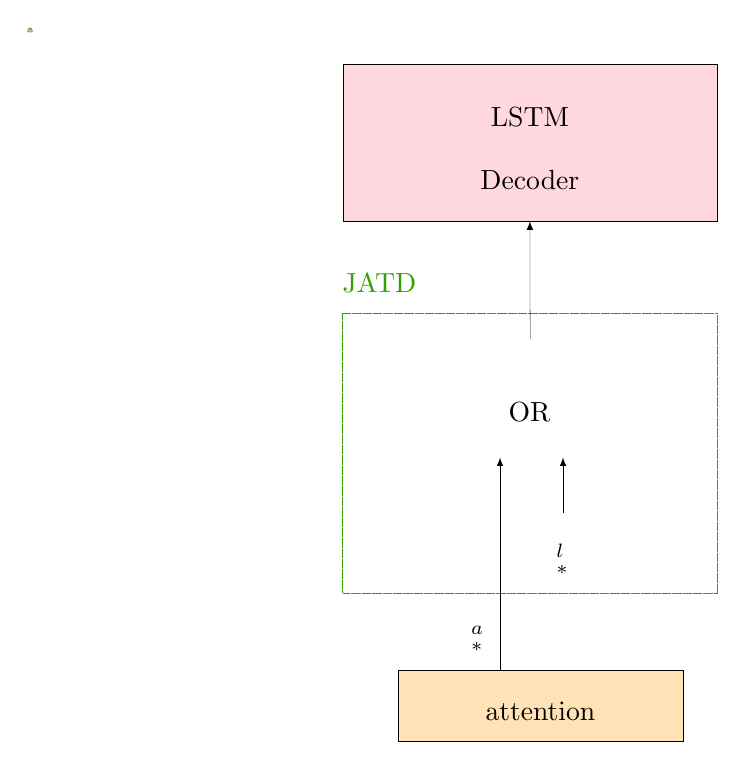
\begin{tikzpicture}[even odd rule]
\pgftransformxscale{1.000000}
\pgftransformyscale{-1.000000}
\definecolor{dialinecolor}{rgb}{0.000000, 0.000000, 0.000000}
\pgfsetstrokecolor{dialinecolor}
\pgfsetstrokeopacity{1.000000}
\definecolor{diafillcolor}{rgb}{1.000000, 1.000000, 1.000000}
\pgfsetfillcolor{diafillcolor}
\pgfsetfillopacity{1.000000}
\pgfsetlinewidth{0.100000\du}
\pgfsetdash{{0.200000\du}{0.200000\du}}{0\du}
\pgfsetmiterjoin
{\pgfsetcornersarced{\pgfpoint{0.000000\du}{0.000000\du}}\definecolor{diafillcolor}{rgb}{0.000000, 0.000000, 0.000000}
\pgfsetfillcolor{diafillcolor}
\pgfsetfillopacity{0.000000}
\fill (4.200000\du,3.763660\du)--(4.200000\du,7.317587\du)--(8.958597\du,7.317587\du)--(8.958597\du,3.763660\du)--cycle;
}{\pgfsetcornersarced{\pgfpoint{0.000000\du}{0.000000\du}}\definecolor{dialinecolor}{rgb}{0.192157, 0.627451, 0.000000}
\pgfsetstrokecolor{dialinecolor}
\pgfsetstrokeopacity{1.000000}
\draw (4.200000\du,3.763660\du)--(4.200000\du,7.317587\du)--(8.958597\du,7.317587\du)--(8.958597\du,3.763660\du)--cycle;
}% setfont left to latex
\definecolor{dialinecolor}{rgb}{0.192157, 0.627451, 0.000000}
\pgfsetstrokecolor{dialinecolor}
\pgfsetstrokeopacity{1.000000}
\definecolor{diafillcolor}{rgb}{0.192157, 0.627451, 0.000000}
\pgfsetfillcolor{diafillcolor}
\pgfsetfillopacity{1.000000}
\node[anchor=base east,inner sep=0pt, outer sep=0pt,color=dialinecolor] at (8.608597\du,5.734686\du){};
\pgfsetlinewidth{0.100000\du}
\pgfsetdash{}{0pt}
\pgfsetmiterjoin
\pgfsetbuttcap
\definecolor{diafillcolor}{rgb}{0.631373, 0.858824, 0.533333}
\pgfsetfillcolor{diafillcolor}
\pgfsetfillopacity{1.000000}
\definecolor{dialinecolor}{rgb}{0.000000, 0.000000, 0.000000}
\pgfsetstrokecolor{dialinecolor}
\pgfsetstrokeopacity{1.000000}
\pgfpathmoveto{\pgfpoint{7.377110\du}{5.600000\du}}
\pgfpathcurveto{\pgfpoint{6.843780\du}{5.600000\du}}{\pgfpoint{6.310440\du}{5.600000\du}}{\pgfpoint{5.777110\du}{5.600000\du}}
\pgfpathcurveto{\pgfpoint{5.777110\du}{5.000000\du}}{\pgfpoint{5.777110\du}{4.100000\du}}{\pgfpoint{6.577110\du}{4.100000\du}}
\pgfpathcurveto{\pgfpoint{7.377110\du}{4.100000\du}}{\pgfpoint{7.377110\du}{5.000000\du}}{\pgfpoint{7.377110\du}{5.600000\du}}
\pgfpathclose
\pgfusepath{fill,stroke}
\pgfsetlinewidth{0.100000\du}
\pgfsetdash{}{0pt}
\pgfsetmiterjoin
{\pgfsetcornersarced{\pgfpoint{0.000000\du}{0.000000\du}}\definecolor{diafillcolor}{rgb}{1.000000, 0.843137, 0.870588}
\pgfsetfillcolor{diafillcolor}
\pgfsetfillopacity{1.000000}
\fill (4.201490\du,0.600000\du)--(4.201490\du,2.600000\du)--(8.957108\du,2.600000\du)--(8.957108\du,0.600000\du)--cycle;
}{\pgfsetcornersarced{\pgfpoint{0.000000\du}{0.000000\du}}\definecolor{dialinecolor}{rgb}{0.000000, 0.000000, 0.000000}
\pgfsetstrokecolor{dialinecolor}
\pgfsetstrokeopacity{1.000000}
\draw (4.201490\du,0.600000\du)--(4.201490\du,2.600000\du)--(8.957108\du,2.600000\du)--(8.957108\du,0.600000\du)--cycle;
}% setfont left to latex
\definecolor{dialinecolor}{rgb}{0.000000, 0.000000, 0.000000}
\pgfsetstrokecolor{dialinecolor}
\pgfsetstrokeopacity{1.000000}
\definecolor{diafillcolor}{rgb}{0.000000, 0.000000, 0.000000}
\pgfsetfillcolor{diafillcolor}
\pgfsetfillopacity{1.000000}
\node[anchor=base,inner sep=0pt, outer sep=0pt,color=dialinecolor] at (6.579299\du,1.394062\du){LSTM};
% setfont left to latex
\definecolor{dialinecolor}{rgb}{0.000000, 0.000000, 0.000000}
\pgfsetstrokecolor{dialinecolor}
\pgfsetstrokeopacity{1.000000}
\definecolor{diafillcolor}{rgb}{0.000000, 0.000000, 0.000000}
\pgfsetfillcolor{diafillcolor}
\pgfsetfillopacity{1.000000}
\node[anchor=base,inner sep=0pt, outer sep=0pt,color=dialinecolor] at (6.579299\du,2.194063\du){Decoder};
\pgfsetlinewidth{0.100000\du}
\pgfsetdash{}{0pt}
\pgfsetbuttcap
{
\definecolor{diafillcolor}{rgb}{0.000000, 0.000000, 0.000000}
\pgfsetfillcolor{diafillcolor}
\pgfsetfillopacity{1.000000}

\pgfsetarrowsend{latex}
\definecolor{dialinecolor}{rgb}{0.000000, 0.000000, 0.000000}
\pgfsetstrokecolor{dialinecolor}
\pgfsetstrokeopacity{1.000000}
\draw (6.583080\du,4.096640\du)--(6.579300\du,2.600000\du);
}
% setfont left to latex
\definecolor{dialinecolor}{rgb}{0.192157, 0.627451, 0.000000}
\pgfsetstrokecolor{dialinecolor}
\pgfsetstrokeopacity{1.000000}
\definecolor{diafillcolor}{rgb}{0.192157, 0.627451, 0.000000}
\pgfsetfillcolor{diafillcolor}
\pgfsetfillopacity{1.000000}
\node[anchor=base west,inner sep=0pt,outer sep=0pt,color=dialinecolor] at (4.200000\du,3.500000\du){JATD};
\pgfsetlinewidth{0.100000\du}
\pgfsetdash{}{0pt}
\pgfsetbuttcap
{
\definecolor{diafillcolor}{rgb}{0.000000, 0.000000, 0.000000}
\pgfsetfillcolor{diafillcolor}
\pgfsetfillopacity{1.000000}

\pgfsetarrowsend{latex}
\definecolor{dialinecolor}{rgb}{0.000000, 0.000000, 0.000000}
\pgfsetstrokecolor{dialinecolor}
\pgfsetstrokeopacity{1.000000}
\draw (6.200000\du,8.300000\du)--(6.200000\du,5.600000\du);
}
\pgfsetlinewidth{0.100000\du}
\pgfsetdash{}{0pt}
\pgfsetbuttcap
{
\definecolor{diafillcolor}{rgb}{0.000000, 0.000000, 0.000000}
\pgfsetfillcolor{diafillcolor}
\pgfsetfillopacity{1.000000}

\pgfsetarrowsend{latex}
\definecolor{dialinecolor}{rgb}{0.000000, 0.000000, 0.000000}
\pgfsetstrokecolor{dialinecolor}
\pgfsetstrokeopacity{1.000000}
\draw (7.000000\du,6.300000\du)--(7.000000\du,5.600000\du);
}
\pgfsetlinewidth{0.000000\du}
\pgfsetdash{}{0pt}
\pgfsetmiterjoin
{\pgfsetcornersarced{\pgfpoint{0.000000\du}{0.000000\du}}\definecolor{diafillcolor}{rgb}{0.000000, 0.000000, 0.000000}
\pgfsetfillcolor{diafillcolor}
\pgfsetfillopacity{0.000000}
\fill (1.611430\du,7.088820\du)--(1.611430\du,8.488820\du)--(6.202015\du,8.488820\du)--(6.202015\du,7.088820\du)--cycle;
}{\pgfsetcornersarced{\pgfpoint{0.000000\du}{0.000000\du}}\definecolor{dialinecolor}{rgb}{0.000000, 0.000000, 0.000000}
\pgfsetstrokecolor{dialinecolor}
\pgfsetstrokeopacity{0.000000}
\draw (1.611430\du,7.088820\du)--(1.611430\du,8.488820\du)--(6.202015\du,8.488820\du)--(6.202015\du,7.088820\du)--cycle;
}% setfont left to latex
\definecolor{dialinecolor}{rgb}{0.000000, 0.000000, 0.000000}
\pgfsetstrokecolor{dialinecolor}
\pgfsetstrokeopacity{1.000000}
\definecolor{diafillcolor}{rgb}{0.000000, 0.000000, 0.000000}
\pgfsetfillcolor{diafillcolor}
\pgfsetfillopacity{1.000000}
\node[anchor=base east,inner sep=0pt, outer sep=0pt,color=dialinecolor] at (6.002015\du,7.982882\du){$\vc_*^a$};
\pgfsetlinewidth{0.000000\du}
\pgfsetdash{}{0pt}
\pgfsetmiterjoin
{\pgfsetcornersarced{\pgfpoint{0.000000\du}{0.000000\du}}\definecolor{diafillcolor}{rgb}{0.000000, 0.000000, 0.000000}
\pgfsetfillcolor{diafillcolor}
\pgfsetfillopacity{0.000000}
\fill (5.400000\du,6.400000\du)--(5.400000\du,7.200000\du)--(8.592500\du,7.200000\du)--(8.592500\du,6.400000\du)--cycle;
}{\pgfsetcornersarced{\pgfpoint{0.000000\du}{0.000000\du}}\definecolor{dialinecolor}{rgb}{0.000000, 0.000000, 0.000000}
\pgfsetstrokecolor{dialinecolor}
\pgfsetstrokeopacity{0.000000}
\draw (5.400000\du,6.400000\du)--(5.400000\du,7.200000\du)--(8.592500\du,7.200000\du)--(8.592500\du,6.400000\du)--cycle;
}% setfont left to latex
\definecolor{dialinecolor}{rgb}{0.000000, 0.000000, 0.000000}
\pgfsetstrokecolor{dialinecolor}
\pgfsetstrokeopacity{1.000000}
\definecolor{diafillcolor}{rgb}{0.000000, 0.000000, 0.000000}
\pgfsetfillcolor{diafillcolor}
\pgfsetfillopacity{1.000000}
\node[anchor=base,inner sep=0pt, outer sep=0pt,color=dialinecolor] at (6.996250\du,6.994063\du){$\vc_*^l$};
\pgfsetlinewidth{0.100000\du}
\pgfsetdash{}{0pt}
\pgfsetmiterjoin
{\pgfsetcornersarced{\pgfpoint{0.000000\du}{0.000000\du}}\definecolor{diafillcolor}{rgb}{1.000000, 0.886275, 0.713726}
\pgfsetfillcolor{diafillcolor}
\pgfsetfillopacity{1.000000}
\fill (4.900000\du,8.300000\du)--(4.900000\du,9.200000\du)--(8.525688\du,9.200000\du)--(8.525688\du,8.300000\du)--cycle;
}{\pgfsetcornersarced{\pgfpoint{0.000000\du}{0.000000\du}}\definecolor{dialinecolor}{rgb}{0.000000, 0.000000, 0.000000}
\pgfsetstrokecolor{dialinecolor}
\pgfsetstrokeopacity{1.000000}
\draw (4.900000\du,8.300000\du)--(4.900000\du,9.200000\du)--(8.525688\du,9.200000\du)--(8.525688\du,8.300000\du)--cycle;
}% setfont left to latex
\definecolor{dialinecolor}{rgb}{0.000000, 0.000000, 0.000000}
\pgfsetstrokecolor{dialinecolor}
\pgfsetstrokeopacity{1.000000}
\definecolor{diafillcolor}{rgb}{0.000000, 0.000000, 0.000000}
\pgfsetfillcolor{diafillcolor}
\pgfsetfillopacity{1.000000}
\node[anchor=base,inner sep=0pt, outer sep=0pt,color=dialinecolor] at (6.712844\du,8.944063\du){attention};
\pgfsetlinewidth{0.100000\du}
\pgfsetdash{}{0pt}
\pgfsetmiterjoin
{\pgfsetcornersarced{\pgfpoint{0.000000\du}{0.000000\du}}\definecolor{diafillcolor}{rgb}{1.000000, 0.843137, 0.870588}
\pgfsetfillcolor{diafillcolor}
\pgfsetfillopacity{0.000000}
\fill (5.833830\du,4.173760\du)--(5.833830\du,5.726926\du)--(7.318673\du,5.726926\du)--(7.318673\du,4.173760\du)--cycle;
}{\pgfsetcornersarced{\pgfpoint{0.000000\du}{0.000000\du}}\definecolor{dialinecolor}{rgb}{0.000000, 0.000000, 0.000000}
\pgfsetstrokecolor{dialinecolor}
\pgfsetstrokeopacity{0.000000}
\draw (5.833830\du,4.173760\du)--(5.833830\du,5.726926\du)--(7.318673\du,5.726926\du)--(7.318673\du,4.173760\du)--cycle;
}% setfont left to latex
\definecolor{dialinecolor}{rgb}{0.000000, 0.000000, 0.000000}
\pgfsetstrokecolor{dialinecolor}
\pgfsetstrokeopacity{1.000000}
\definecolor{diafillcolor}{rgb}{0.000000, 0.000000, 0.000000}
\pgfsetfillcolor{diafillcolor}
\pgfsetfillopacity{1.000000}
\node[anchor=base,inner sep=0pt, outer sep=0pt,color=dialinecolor] at (6.576252\du,5.144406\du){OR};
\end{tikzpicture}

}
\end{center}
\caption[]{\label{fig:las_jatd} Details of JATD implementation. The ``JATD'' block can be added to the outputs of either attention block in fig. \ref{fig:delib}.
}
\end{figure}

LAS-JATD \cite{sainath2020jatd} augments LAS to enable training on paired audio-text data, as well as unpaired (i.e. text-only) data. This is done through the introduction of a new learnable fixed context vector, $\vc_e^l$, which is used as an alternative to the acoustic context vector $\vc_e^a$ (fig. \ref{fig:las_jatd}). During inference, two log probabilities are produced, one based on $\vc_e^a$ and the other based on $\vc_e^l$. These are interpolated using weight $\lambda$ to produce the final output log probabilities:

\begin{equation}
\label{eq:las_jatd_probs}
\lambda \log{p(\vy_u^d |\vx, \vc_e^a , \vy_{u - 1:1}^d )} + (1 - \lambda)\log{p(\vy_u^d | \vc_e^l , \vy_{u-1:1}^d )}
\end{equation}

The first term in this equation represents the familiar acoustic model (i.e. a regular two-pass LAS). The second term, $\log{p(\vy_u^d | \vc_e^l , \vy_{u-1:1}^d )}$, can be thought of as a language model since it does not depend on acoustic features, $\vx$.

LAS-JATD also provides a framework for incorporating unpaired data into training (eq. \ref{eq:las_jatd_loss}). It uses both acoustic and learnable context vectors when training on both paired and unpaired data. Acoustic context vectors are generated based on real audio, $\vx^a \in \vx$, for paired examples and ``created'' audio, $\vx^l \in \vx$, for unpaired examples. Importantly, it restricts training so only paired examples update the encoder attention parameters and only unpaired examples update the fixed context vector. This avoids biasing acoustic attention parameters towards unpaired data, and was found to be effective in \cite{sainath2020jatd}. In this work, we explore synthesizing audio based on text data to create $\vx^l$.

\begin{equation}
\label{eq:las_jatd_loss}
  \mathcal{L} =
    \begin{cases}
      \lambda \log{p(\vy_u^d |\vx^a, \vc_e^a , \vy_{u - 1:1}^d )} + (1 - \lambda)\log{p(\vy_u^d | \vc_e^l , \vy_{u-1:1}^d )}\\
      \text{if paired example}\\
      \lambda \log{p(\vy_u^d |\vx^l, \vc_e^a , \vy_{u - 1:1}^d )} + (1 - \lambda)\log{p(\vy_u^d | \vc_e^l , \vy_{u-1:1}^d )}\\
      \text{if unpaired example}\\
    \end{cases} 
\end{equation}

LAS-JATD improves performance through the addition of unpaired data to its training set, but misses out on gains from the spell-correcting capabilities of deliberation models.

\subsection{Proposed Method: Deliberation-JATD
\label{sec:methods_delib_jatd}}

We propose the Deliberation-JATD model, combining deliberation's spell-correcting benefits with JATD's ability to train on unpaired data. Similar to LAS-JATD, this model uses fixed context vectors as an alternative to attention context vectors, $c_e^a$ and $c_b^a$. This results in a new set of output log probabilities that act as a language model.

Given that deliberation models contain two attention contexts, we examine two Deliberation-JATD variations. The first, dubbed ``partial JATD'', uses the fixed context vector $\vc_e^l$ as an alternative to the encoder attention context, $\vc_e^a$, while continuing to use first-pass decoder context, $\vc_b^a$. This results in the LM log probabilities, $\log{p(\vy_u^d |\vx, \vc_e^l , \vc_b^a, \vy_{u - 1:1}^d )}$, and the following final model outputs used during inference:

\begin{equation}
\label{eq:deliberation_partial_jatd_probs}
\lambda \log{p(\vy_u^d |\vx, \vc_e^a , \vc_b^a, \vy_{u - 1:1}^d )} + (1 - \lambda)\log{p(\vy_u^d |\vx, \vc_e^l , \vc_b^a, \vy_{u - 1:1}^d )}
\end{equation}

The second variant, named ``full JATD'', goes one step further and adds a second fixed context vector, $\vc_b^l$, as an alternative to its first pass decoder attention context, $\vc_b^a$ (eq. \ref{eq:deliberation_full_jatd_probs}). This means that both attention contexts are replaced and the LM log probabilities having no dependence on the acoustic inputs, $\vx$.

\begin{equation}
\label{eq:deliberation_full_jatd_probs}
\lambda \log{p(\vy_u^d |\vx, \vc_e^a , \vc_b^a, \vy_{u - 1:1}^d )} + (1 - \lambda)\log{p(\vy_u^d | \vc_e^l , \vc_b^l, \vy_{u - 1:1}^d )}
\end{equation}

We use the ``joint'' training strategy \cite{sainath2020jatd} to train both variants on a mix of supervised audio and text-only data paired with TTS audio. The resulting training loss is similar to eq. \ref{eq:las_jatd_loss}, but incorporates eq. \ref{eq:deliberation_partial_jatd_probs} or eq. \ref{eq:deliberation_full_jatd_probs} for the unpaired text term, depending on the model variation used. Similar to LAS-JATD, we distinguish between real audio from paired data, $\vx^a$, and synthetic audio from text data, $\vx^l$, and only backpropagate some parameters for each type of data. Specifically, encoder attention parameters are held constant for synthetic audio and the fixed attention context vectors are held constant for real audio. The second-pass decoder parameters are updated for both types of data.

Full JATD's LM is similar to LAS-JATD's LM in that it replaces all attention contexts (from the encoder and first-pass decoder) with fixed vectors. This means that the LM component's second-pass decoder completely ignores the first-pass decoder and all acoustic information. As a result, the LM learns to spell-correct based purely on previous model outputs, $\vy_{u - 1:1}^d$. In contrast, partial JATD was designed to more frequently expose the second-pass decoder to the first-pass decoder during training. Its LM keeps the first-pass decoder attention context, allowing the second-pass decoder to train with it and the LM to make use of some indirect acoustic information.

\subsection{Training
\label{sec:methods_training}}

All models were initialized from an RNN-T trained with supervised audio-text paired data. The same model was also used as the baseline RNN-T model when analyzing performance. All training sets that included TTS used a mix of 90\% audio-text pairs and 10\% pure text data with corresponding TTS. We will refer to this training set as the ``mixed audio'' training set. For all JATD models, an interpolation weight of $\lambda = 0.1$ was found to work well in training.
